\section{Théorie de Griffith: essai \textit{End-Notched Flexure} (ENF)}


L'essai ENF (End-Notched Flexure) consiste en une flexion 3 points d'une poutre entaillée à mi-hauteur par une préfissure de longueur initiale $a_0$ débouchant à une des extrémités de la poutre (Figure \ref{fig:ENF}). Cet essai est notamment utilisé pour caractériser les propriétés de délaminage d'interface des matériaux composites multicouches.

La poutre de longueur $L$, de hauteur $2h$ et de largeur $b$, est simplement appuyée à ses extrémités et chargée par un effort ponctuel vertical $F$ appliqué au centre de la poutre. On note $q$ le déplacement vertical du point d'application de la force et $Q = F/b$ l'intensité de la force par unité de largeur. Une expression analytique approchée de la relation force/déplacement peut-être obtenue à l'aide d'une modélisation simplifiée reposant sur la théorie des poutres d'Euler-Bernoulli \cite{allix1995damage}. Pour une fissure de taille $a$ fixée, la relation force/déplacement s'exprime comme:
\begin{equation}
q = \begin{cases}
\dfrac{L^3/12 + a^3}{32D}Q & \text{si } a\leq L/2\\
\dfrac{L^3/3 - (L-a)^3}{32D}Q & \text{si } a\geq L/2
\end{cases}
\end{equation}
où $D = E h^3/12$ est la raideur en flexion d'une moitié de poutre par unité de largeur.


\begin{figure}[h]
\begin{center}
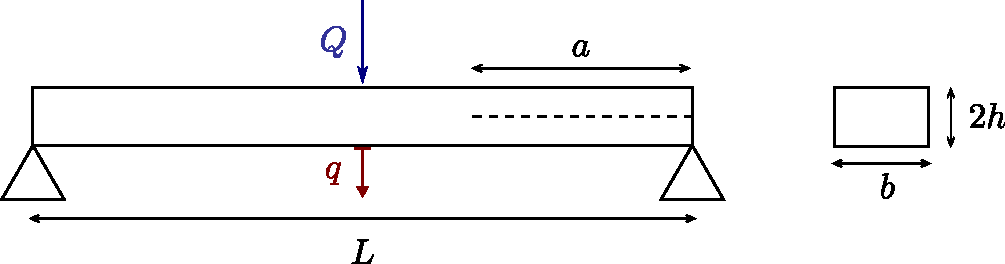
\includegraphics[width=0.8\textwidth]{ENF}
\end{center}
\caption{Essai ENF}\label{fig:ENF}
\end{figure}

\begin{questions}
\setcounter{question}{-1}
\question Quel est le mode principal de sollicitation de la fissure ?
\begin{solution}
Sur appui, la fissure est sollicitée principalement par des contraintes de cisaillement, soit une fissuration en mode II. On pourra faire remarquer que la fissure est également soumise à des contraintes de compression. Dans le cas de poutres très élancées ($h \ll L$), celles-ci sont en général de faible amplitude vis-à-vis des contraintes de cisaillement.
\end{solution}
\end{questions}

\subsection{Rappels préliminaires}
\begin{questions}

\question On note $S(a)=q/Q$ la souplesse de la structure par unité de largeur, à longueur $a$ de fissure fixée. Donner la valeur de l'énergie potentielle $\mathcal{P}$ (par unité de largeur) de la solution suivant que l'on pilote: (a) en force, (b) en déplacement.
\begin{solution}
Par définition de la souplesse, l'énergie élastique par unité de largeur vaut:
$$E_\text{el}=\dfrac{1}{2}S(a)Q^2$$
Lorsque l'on pilote en force, on donc:
$$\mathcal{P} = E_\text{el}-W_\text{ext} = \dfrac{1}{2}S(a)Q^2 - Qq = -\dfrac{1}{2}S(a)Q^2$$
tandis que si l'on pilote en déplacement:
on a:
$$\mathcal{P} = E_\text{el} = \dfrac{1}{2}S(a)Q^2 = \dfrac{1}{2}\dfrac{q^2}{S(a)}$$
notons que dans ce cas, on a réexprimé l'énergie potentielle en fonction du paramètre de chargement, ici le déplacement $q$.
\end{solution}
\question En déduire le taux de resitution d'énergie $\mathcal{G}$ dans les deux modes de pilotage de chargement.
\begin{solution}
De manière générale:
$$\mathcal{G} = -\dfrac{d\mathcal{P}}{da} $$
On a alors pour un pilotage en force:
$$\mathcal{G} =  \dfrac{1}{2}S'(a)Q^2$$
et pour un pilotage en déplacement:
$$\mathcal{G} =  \dfrac{1}{2}S'(a)\left(\dfrac{q}{S(a)}\right)^2=\dfrac{1}{2}S'(a)Q(a)^2$$
\end{solution}
\question Rappeler la condition de propagation et de stabilité/instabilité de propagation de la fissure.
\begin{solution}
Il y a propagation lorsque $\mathcal{G}=\mathcal{G}_c$. La propagation sera stable si $\mathcal{G}'(a) < 0$ tandis qu'elle sera instable sinon.
\end{solution}
\end{questions}

\subsection{Application à l'essai ENF: pilotage en force}
Dans cette section, on se limite au \textbf{pilotage en force}.

\begin{questions}
\setcounter{question}{3}
\question Dans le cas $a\leq L/2$, déterminer la condition de propagation de la fissure. Discuter du caractère stable ou instable de la propagation.
\begin{solution}
On a ici:

$$S'(a) = \dfrac{3a^2}{32 D} \quad \text{soit } \mathcal{G}=\dfrac{3Q^2a^2}{64D}$$
Ainsi, la fissure ne se propage pas tant que:
$$Q \leq Q_c = \sqrt{\dfrac{64D\mathcal{G}_c}{3a_0^2}}$$
Au delà de $Q_c$, comme $\mathcal{G}'(a_0) >0$, la propagation est instable.
\end{solution}
\question Faire de même pour le cas $a \geq L/2$.
\begin{solution}
On a dans ce cas:
$$S'(a) = \dfrac{3(L-a)^2}{32D} \quad \text{soit } \mathcal{G}=\dfrac{3Q^2(L-a)^2}{64D}$$
Ainsi, la fissure ne se propage pas tant que:
$$Q \leq Q_c = \sqrt{\dfrac{64D\mathcal{G}_c}{3(L-a_0)^2}}$$
Au delà de $Q_c$, comme 
$$\mathcal{G}'(a_0) =  -\dfrac{6Q^2(L-a_0)}{64D}<0,$$ la propagation est stable.
\end{solution}
\end{questions}

\subsection{Application à l'essai ENF: pilotage en déplacement}

Dans cette section, on se limite au \textbf{pilotage en déplacement} et au cas $a\leq L/2$.

\begin{questions}
\setcounter{question}{5}
\question Déterminer la condition de propagation de la fissure. 
\begin{solution}
On a toujours:
$$S'(a) = \dfrac{3a^2}{32D} \quad \text{soit } \mathcal{G}=48Dq^2\dfrac{a^2}{(L^3/12+a^3)^2}$$
Ainsi, la fissure ne se propage pas tant que:
$$q \leq q_c = \sqrt{\dfrac{\mathcal{G}_c}{48D}}\dfrac{L^3/12+a_0^3}{a_0}$$
\end{solution}
\question Discuter du caractère stable ou instable de la propagation. On pourra pour cela s'appuyer sur le graphe de la fonction $f(x) = \dfrac{x^2}{(1/12+x^3)^2}$ représenté sur la Figure \ref{fig:graphe-fonction}.
\begin{figure}
\begin{center}
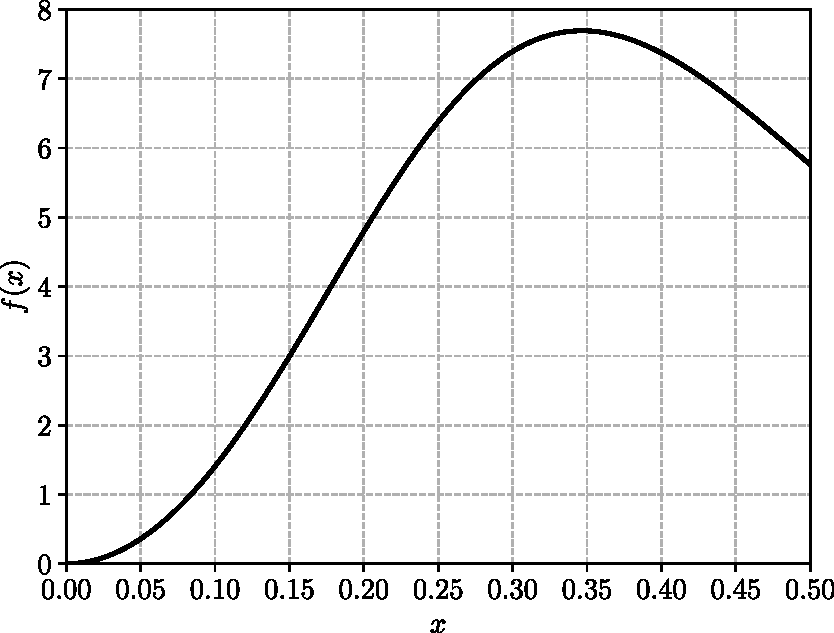
\includegraphics[width=0.5\textwidth]{function_variation}
\end{center}
\caption{Graphe de la fonction $f(x) = \dfrac{x^2}{(1/12+x^3)^2}$}\label{fig:graphe-fonction}
\end{figure}
\begin{solution}
Au delà de $q_c$, la stabilité est conditionnée par le signe de $\mathcal{G}'(a_0)$ qui est lié au signe de $f'(a_0/L)$ pour la fonction $f$ indiquée par l'énoncé. Graphiquement, on trouve que cette dérivée est positive si $a_0/L < 0.35$ environ, correspondant à une propagation instable. Pour des fissures initialement plus grandes que $0.35L$ la propagation est stable.

Notons que l'étude de variation exacte de la fonction conduit à la condition $a_0 \geq \left(\frac{1}{24}\right)^{1/3}L \approx 0.347L$. Ces différentes conditions de stabilité se traduisent également dans l'évolution de la courbe force/déplacement suivant la taille de la préfissure.

\begin{R_figure}
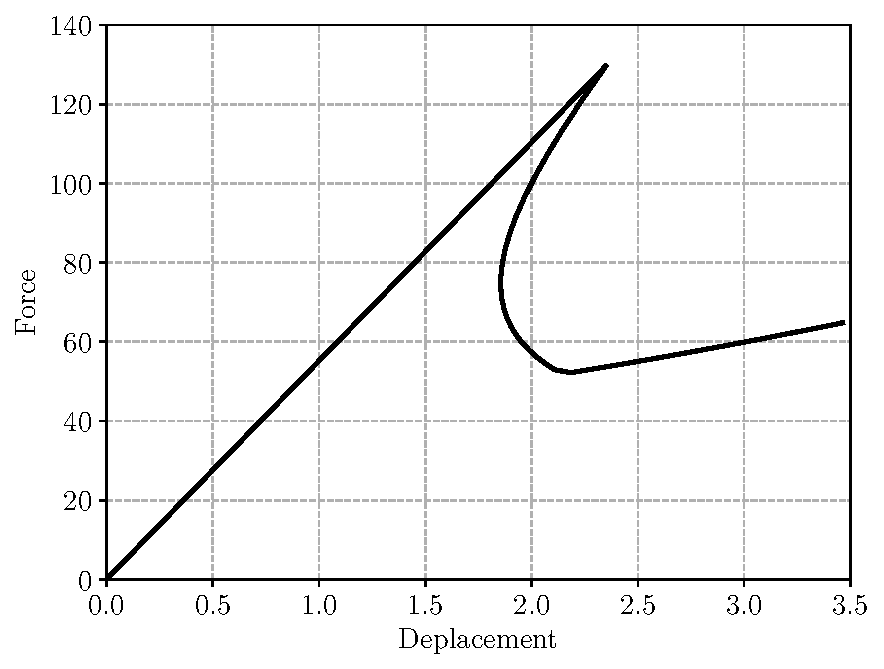
\includegraphics[width=0.49\textwidth]{ENF_force_deplacement_0.2L}
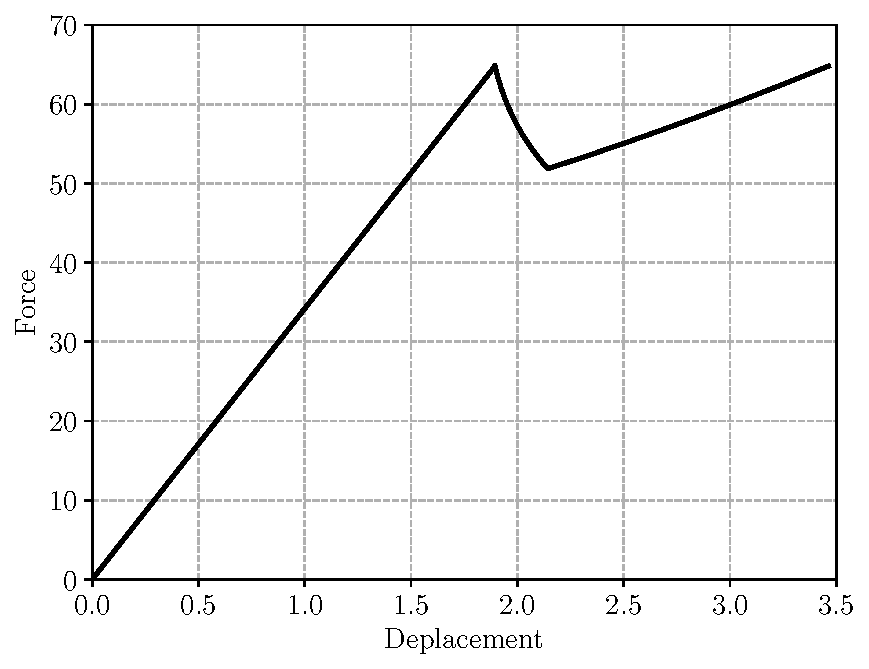
\includegraphics[width=0.49\textwidth]{ENF_force_deplacement_0.4L}\\
\captionof{figure}{Force/déplacement à déplacement contrôlé pour différentes longueurs initiales de fissure. Gauche: $a_0=0.2L$ (instable); droite: $a_0=0.4L$ (stable)}
\end{R_figure}

\end{solution}
\end{questions}
